% !TeX program = pdflatex
\documentclass[conference]{IEEEtran}

\usepackage{verbatim}
\DeclareMathAlphabet{\mathpzc}{OT1}{pzc}{m}{it}
\usepackage{multirow}
\usepackage{amsmath,amssymb,amsfonts}
\usepackage[
top    = 0.7in,
bottom = 1in,
left   = 0.65in,
right  = 0.59in]{geometry}
\usepackage{graphicx}
\usepackage{textcomp}
\usepackage{xcolor}
\colorlet{blue}{black}
\usepackage{url}
\usepackage{float}
\restylefloat{figure}
\usepackage[ruled,vlined,linesnumbered]{algorithm2e}
\floatname{algorithm}{}


\begin{document}

\title{AntiFLipper: A Secure and Efficient Defense Against Label-Flipping Attacks in Federated Learning}

\author{\IEEEauthorblockN{Aashnan Rahman$^{1}$, Abid Hasan$^{2}$, Sherajul Arifin$^{3}$, Faisal Haque Bappy$^{4}$, Tahrim Hossain$^{5}$,\\ Tariqul Islam$^{6}$, Abu Raihan Mostofa Kamal$^{7}$, and Md. Azam Hossain$^{8}$}

\IEEEauthorblockA{
$^{1, 2, 7, 8}$ Islamic University of Technology, Bangladesh.\\
$^{3}$ United International University, Bangladesh.\\
$ ^{4, 5, 6}$ Syracuse University, United States.\\
Email: \{aashnanrahman@iut-dhaka, abidhasan32@iut-dhaka, sherajul@cse.uiu.ac.bd,\\ fbappy@syr, mhossa22@syr, mtislam@syr, azam@iut-dhaka, raihan.kamal@iut-dhaka\}.edu} 
}

\maketitle
\pagestyle{empty}

\begin{abstract}
Federated learning (FL) enables decentralized model training without centralizing clients' raw data, but remains vulnerable to label-flipping attacks in which malicious clients corrupt local labels to poison the global model. We introduce AntiFLipper, a computationally efficient defense against multi-class label flipping under a threat model restricted to local label manipulation: attackers cannot falsify model updates, tamper with the evaluation procedure, or compromise the server. AntiFLipper evaluates the global model on each client's local data and sends one scalar accuracy score to the server, which uses relative deviations to update trust and filter persistently anomalous clients. Experiments on MNIST and CIFAR-10 under IID and Dirichlet non-IID partitions show accuracy comparable to the evaluated defenses while substantially reducing server-side aggregation time. AntiFLipper therefore offers a lightweight security--efficiency trade-off for label-flipping defense; evaluation on genuinely resource-constrained hardware remains future work.
\end{abstract}

\begin{IEEEkeywords}
Federated Learning, Label Flipping Attack, Malicious Node Detection, Attack Mitigation, IoT, Edge Networks
\end{IEEEkeywords}


\section{Introduction}

\textcolor{blue}{Federated learning (FL) has emerged as a prominent distributed learning paradigm for communication networks and edge computing systems, enabling geographically dispersed clients such as mobile devices, IoT sensors, and edge devices to collaboratively train a global model without sharing raw data~\cite{fedavg-pmlr-v54-mcmahan17a,li2020federated}. By exchanging model updates rather than raw records, FL supports data minimization, although it does not by itself guarantee privacy~\cite{kairouz2021advances,lyu2020threats}. Its decentralized nature also exposes it to data-poisoning attacks, among which \textit{label-flipping attacks} are particularly relevant to networked deployments. In this attack, malicious clients deliberately mislabel their local training data before submitting normally trained updates. Our threat model restricts the attacker to this local label manipulation: the attacker cannot directly modify the resulting update, intercept communications, or access server or peer data. Despite this simplicity, compromised clients can substantially degrade the global model~\cite{biggio2011support,tolpegin2020data}, threatening the reliability of FL-enabled distributed systems.} 

Existing defenses typically rely on server-side anomaly detection or robust aggregation, requiring the server to inspect, cluster, or compare client updates~\cite{nguyen2022flame,yin2018byzantine,NIPS2017_f4b9ec30}. \textcolor{blue}{This can introduce substantial server-side computation and, in methods such as FLTrust, an additional assumption that the server owns a small clean labeled dataset~\cite{cao2020fltrust}. Other defenses can degrade under non-IID data distributions prevalent in heterogeneous wireless networks~\cite{fung2020limitations}.}

\textcolor{blue}{To address these limitations, we propose AntiFLipper, a defense that shifts detection to the client side through local accuracy evaluation, avoiding server-side model inspection entirely. Unlike approaches that depend on server-held reference data or expensive cryptographic mechanisms, AntiFLipper infers trust from relative client performance deviations, making it well-suited for resource-constrained edge and IoT deployments.}

The core contributions of this paper are:

\begin{itemize}
   \item \textbf{Attack Detection \& Mitigation:} We propose AntiFLipper, a novel trust-based weighted aggregation method that detects and mitigates multi-class label-flipping attacks by identifying and excluding malicious clients, even in dynamic attack scenarios.

   \item \textbf{Accuracy and Efficiency:} AntiFLipper matches or exceeds state-of-the-art defenses in accuracy while achieving significantly lower aggregation time by avoiding server-side model update inspection.

   \item \textbf{Improved Scalability:} By shifting detection to client devices, AntiFLipper minimizes server burden, improving scalability in large-scale decentralized networks.
    
    %\item \textcolor{blue}{\textbf{Privacy-Preserving Client-Side Evaluation:} AntiFLipper relies on a trusted client-side evaluation module that shares only a scalar accuracy value with the server---no raw data or model gradients are exposed---enabling robust detection without any server-held reference data.}
\end{itemize}


    The remainder of the paper is structured as follows. In Section \ref{sec:problem Statement}, we describe the problem statement and our research objectives. In Section \ref{sec:relatedworks}, we review existing work related to the detection and defense against label-flipping attacks by malicious clients in federated learning scenarios. In Section \ref{sec:methodology}, we present AntiFLipper in detail.  In Section \ref{sec:implement&eval} we present system implementation and performance evaluation. In Section \ref{sec:securityanalysis}, we provide a security analysis, discussing the robustness of our approach in mitigating malicious attacks, including its behavior under adaptive and colluding adversaries. In Section \ref{sec:overhead}, we analyze the computational and communication overhead introduced by client-side evaluation. Section~\ref{sec:limitations} discusses the limitations of our approach and threats to validity. Finally, Section \ref{sec:conclusion} summarizes the key findings and concludes the paper.


\section{Problem Statement}
\label{sec:problem Statement}

\subsection{Label Flipping Attack}
Let \(C = \{c_1, c_2, \ldots, c_n\}\) be the set of clients participating in the federated learning process. Each client \( c_i \in C \) possesses a local dataset \(D_i = \{(x_k, y_k)\}_{k=1}^{m_i},\) where \( x_k \in \mathcal{X} \) is the input feature and \( y_k \in \mathcal{Y} \) is the true class label. \textcolor{blue}{In our threat model, the adversary is strictly limited to manipulating its local data (i.e., label-flipping) and has no capability beyond this scope.} In a label-flipping attack, the adversary modifies this dataset into a corrupted version \(D'_i = \{(x_k, y'_k)\}_{k=1}^{m_i},\) such that \( y'_k \neq y_k \) for a substantial subset of the data~\cite{wang2020attack}. These poisoned labels cause the local model \( m'_i \), trained on \( D'_i \), to encode incorrect decision boundaries. A common variant is the \textit{targeted label-flipping attack}, where the adversary selects a source class \( s \in \mathcal{Y} \) and a target class \( \tau \in \mathcal{Y} \), applying:
\[
y'_k =
\begin{cases}
\tau & \text{if } y_k = s, \\
y_k & \text{otherwise.}
\end{cases}
\]
The malicious client then trains locally and submits the resulting model \( m'_i \) to the server. Over time, the aggregation of poisoned updates subtly shifts the global model's decision boundaries toward the adversary's target class~\cite{cao2020fltrust}, \textcolor{blue}{relying solely on local label manipulation} without requiring server access or deviating from the standard FL protocol.

\subsection{Threat Model Boundary and Adaptive Adversaries}
\label{sec:threatext}
\textcolor{blue}{Our primary threat model, consistent with the label-flipping literature~\cite{tolpegin2020data,jebreel2024lfighter}, restricts the adversary to local data manipulation: the attacker cannot tamper with model updates, the evaluation procedure, or server-side computation. This scoping is deliberate, as it isolates the specific and widely-studied threat of label corruption from the broader and largely orthogonal problem of Byzantine gradient manipulation, which is already addressed by a separate line of robust-aggregation work~\cite{yin2018byzantine,NIPS2017_f4b9ec30,mhamdi2018hidden}. We nonetheless discuss two natural extensions of the adversary's capabilities that a reviewer or practitioner may reasonably ask about.}

\textcolor{blue}{\textit{Falsified accuracy reports.} A strictly stronger adversary could additionally misreport its local accuracy $acc_{ij}$ instead of, or in addition to, flipping labels, attempting to mimic $acc_{avg}$ and evade the trust penalty. This capability lies outside our stated threat model (Section~\ref{sec:problem Statement}), since it requires the attacker to tamper with the evaluation/reporting pipeline rather than only the local dataset. It is nonetheless a realistic concern in deployments without secure client attestation. A natural mitigation is for the server to occasionally issue a small \emph{challenge set}, a fixed, previously unseen mini-batch distributed identically to all active clients, and compare each client's self-reported accuracy against the trust-weighted aggregate behavior implied by the client's submitted model update on that same batch; a large mismatch between reported and re-derived accuracy is itself an anomaly signal. We view a full protocol and empirical evaluation of this extension, e.g., via lightweight zero-knowledge proofs of correct local evaluation~\cite{shen2024lfrppfl} or commit-then-reveal accuracy reporting, as important future work rather than a claim made by the present evaluation.}

\textcolor{blue}{\textit{Adaptive and colluding label-flippers.} A more sophisticated adversary could perform a \emph{partial} flip (poisoning only a fraction of local labels) or coordinate with other malicious clients so that each client's accuracy deviation stays near the trust threshold $\tau_{\text{thresh}}$. Such strategies may trade attack impact for detectability, but the present analysis does not establish a quantitative bound on that trade-off. Empirically stress-testing partial-flip and colluding strategies explicitly designed to evade average-based detection is therefore important future work (Section~\ref{sec:limitations}); Propositions~1 and~2 (Section~\ref{sec:securityanalysis}) are conditional analyses rather than guarantees against these adaptive attackers.}

\subsection{Research Objectives}
\textcolor{blue}{Many defenses against label-flipping attacks rely on centralized anomaly detection over high-dimensional client updates, while reference-based approaches impose an additional trusted-data requirement at the server. These design choices can increase server-side cost or deployment assumptions.}
%Existing defenses against label-flipping attacks often rely on centralized anomaly detection at the server, assuming full visibility into client behavior---assumptions that rarely hold in practice. This introduces \textcolor{blue}{performance bottlenecks, negatively affecting scalability and responsiveness}, creates a single point of failure, and contradicts FL's privacy-preserving principles.

To address these challenges, our research pursues the following three core objectives: i) \textit{design a decentralized aggregation method} that accurately detects and mitigates label-flipping attacks; ii) \textit{maintain high model performance} and reduce aggregation time even in the presence of adversarial clients, ensuring both robustness and efficiency; and iii) \textit{shift the majority of computations to the client side} and rigorously analyze the trade-offs in system efficiency, scalability, and resilience under adversarial conditions. Together, these objectives aim to build a trustworthy federated learning framework that resists adversarial manipulation while preserving client privacy and enabling scalable deployment.


\section{Related Work}
\label{sec:relatedworks}

\subsection{Label Flipping-Specific Defenses}
Several approaches have tackled label-flipping attacks in federated learning. Tolpegin et al.~\cite{tolpegin2020data} demonstrated the feasibility of such attacks and proposed a Principal Component Analysis based mechanism to detect malicious clients, but their method lacks generalization guarantees and performs poorly in non-IID settings. Fung et al.~\cite{fung2020limitations} introduced FoolsGold, leveraging cosine similarity between gradient updates. While effective against sybil-style poisoning, it suffers from false positives in non-IID scenarios and incurs high computational cost. 

Nguyen et al.~\cite{nguyen2022flame} proposed FLAME, combining HDBSCAN clustering, differential privacy, and noise addition. It preserves model utility but requires careful tuning and introduces substantial overhead. Jebreel et al.~\cite{jebreel2024lfighter} developed LFighter, reweighting client updates using feature-level centroid deviation. It improves robustness but its effectiveness declines with data heterogeneity.

\textcolor{blue}{Two recent works directly target label-flipping in non-IID FL settings. Li et al.~\cite{li2023hscs} proposed an Honest Score Client Selection Scheme that evaluates clients against a clean server-held dataset. This provides a useful trust anchor but assumes that the server can obtain representative, correctly labeled reference data. Shen et al.~\cite{shen2024lfrppfl} introduced a privacy-preserving defense based on homomorphic encryption and secure aggregation, providing stronger confidentiality guarantees at the cost of cryptographic computation. AntiFLipper instead avoids both a server reference dataset and cryptographic processing, while accepting the narrower threat-model and accuracy-reporting limitations discussed in Sections~\ref{sec:threatext} and~\ref{sec:limitations}.}

\textcolor{blue}{More recent label-flipping-specific defenses have continued to explore client-side and behavior-based detection. Jiang et al.~\cite{jiang2023dataquality} proposed MCDFL, which recovers a latent feature-space distribution to estimate per-client data quality. Ovi et al.~\cite{ovi2023confident} used prediction-confidence statistics to identify label noise, while Li et al.~\cite{li2025flgt} (FLGT) and FedAlign~\cite{fedalign2026} use update similarity or richer feature/distribution statistics to guide trust. Abroshan~\cite{abroshan2025aitoprotect} instead monitors model-output behavior in a general machine-learning pipeline. Relative to these approaches, AntiFLipper's distinguishing design choice is to report a single local accuracy scalar without a server-held reference dataset or server-side inspection of client updates.}

\textcolor{blue}{We note that the accuracy-deviation principle underlying AntiFLipper is conceptually related to prior trust- and validation-score-based defenses such as FLTrust~\cite{cao2020fltrust}, which bootstraps trust from a server-held root dataset, and general Byzantine-robust aggregation rules such as Multi-Krum~\cite{NIPS2017_f4b9ec30}, Bulyan~\cite{mhamdi2018hidden}, and the certified-robustness framework CRFL~\cite{xie2021crfl}, which operate directly on model updates rather than client-reported evaluation scalars. AntiFLipper's novelty relative to this broader family lies specifically in (i) requiring no server-held reference dataset (unlike FLTrust and HSCS~\cite{li2023hscs}), (ii) requiring no inspection of model updates or gradients (unlike Multi-Krum, Bulyan, FLAME, and CRFL), and (iii) transmitting a single scalar rather than a feature or confidence vector (unlike MCDFL~\cite{jiang2023dataquality} and FLGT~\cite{li2025flgt}). Our empirical comparison therefore focuses on defenses designed for, or commonly evaluated against, label-flipping attacks.}


%\textcolor{blue}{Two recent works directly target label-flipping in non-IID FL settings and warrant closer examination. Li et al.~\cite{li2023hscs} proposed an Honest Score Client Selection Scheme that evaluates clients against a clean server-held dataset. While effective in non-IID conditions, this approach requires the server to maintain labeled reference data, which introduces a privacy concern: the reference dataset encodes sensitive distributional information and contradicts the data-minimization principle of FL---the server essentially holds data on behalf of users, violating a core FL premise. Moreover, evaluation is confined to MNIST, and performance on more complex datasets such as CIFAR-10 is not demonstrated, raising questions about generalizability. Shen et al.~\cite{shen2024lfrppfl} introduced a privacy-preserving defense against label-flipping on non-IID data via cryptographic mechanisms. While the privacy guarantees are stronger, the approach incurs significant computational overhead from encryption and secure aggregation protocols, raising scalability concerns for large client populations and resource-constrained edge devices---precisely the deployment scenarios where FL is most valuable. Neither work validates on complex datasets such as CIFAR-10. AntiFLipper avoids these limitations: it requires no server-side reference data, no cryptographic overhead, and demonstrates strong detection performance on both MNIST and CIFAR-10 under IID and non-IID settings.}

% AntiFLipper avoids these limitations: it requires no server-side reference data, no cryptographic overhead, and demonstrates strong detection performance on both MNIST and CIFAR-10 under IID and non-IID settings.}

\subsection{Native Federated Learning Defenses}

While not specifically tailored to counter label-flipping attacks, several robust aggregation methods have been studied in this context. FedAvg\cite{fedavg-pmlr-v54-mcmahan17a}, the popular aggregation mechanism in federated learning, lacks robustness against adversarial updates and suffers significant accuracy degradation under targeted label-flipping. To improve resilience, Yin et al.~\cite{yin2018byzantine} introduced coordinate-wise Median and Trimmed Mean strategies, demonstrating moderate robustness in IID settings but degraded performance in non-IID scenarios. Multi-Krum~\cite{NIPS2017_f4b9ec30} uses distance-based filtering, assuming an IID setting and a known number of adversaries; its performance deteriorates with data heterogeneity and its quadratic complexity limits scalability.

In contrast, our proposed method, AntiFLipper, is designed without relying on data distribution assumptions or prior adversary knowledge. It provides a principled aggregation framework that generalizes well across non-IID environments and varying model architectures. Notably, AntiFLipper significantly reduces computational overhead while maintaining high model accuracy across all evaluated scenarios, making it a practical and scalable solution for real-world federated learning applications where robustness and efficiency are critical.


\section{Detailed Design}
\label{sec:methodology}

%\textcolor{blue}{AntiFLipper defends FL against label-flipping attacks through a lightweight, client-side accuracy evaluation mechanism. The core intuition is that a global model trained predominantly on honest data will yield notably lower accuracy when evaluated on a client's poisoned local data, since flipped label assignments conflict with the model's learned representations. The independent client-side mechanism deployed on each client evaluates the current global model using a subset of the client’s private data and reports only a scalar accuracy value to the server. No raw data or gradients are transmitted, thereby preserving privacy. The server uses these scalars to maintain a per-client trust score, progressively down-weighting and eventually excluding clients with persistently anomalous accuracy. The method does not require explicit knowledge of the data distribution, it relies on \emph{relative} performance deviations among clients, tolerating transient drops due to natural data heterogeneity while penalizing consistently anomalous behavior. Since attackers are restricted to label manipulation only, they cannot interfere with the local evaluation process, an attacker capable of manipulating model updates or the evaluation mechanism would instead be conducting model poisoning, which is a distinct and out-of-scope threat. This design deliberately avoids server-side model update inspection---the dominant overhead source in competing methods, keeping aggregation cost minimal and the framework scalable for resource-constrained edge and IoT deployments.}

\textcolor{blue}{AntiFLipper defends federated learning against label-flipping attacks via a lightweight client-side accuracy-evaluation mechanism. The core intuition is that a global model trained mostly on honest data will exhibit lower accuracy on a client's poisoned data because flipped labels conflict with the learned decision rule. The client-side mechanism independently evaluates the current global model on a subset
of the client's private data and reports only a scalar accuracy to the server, transmitting no additional raw data or gradients. From these scalars, the server maintains a per-client trust score, progressively down-weighting and eventually excluding clients with persistently anomalous accuracy. The method does not require the server to know each client's data distribution; it relies on \emph{relative} performance deviations across clients and uses a multi-round counter to reduce sensitivity to isolated fluctuations. Since attackers are restricted to label manipulation, they cannot affect the evaluation process beyond corrupting the labels on which evaluation is performed. %Attacks involving modification of model updates or the evaluation mechanism correspond to model poisoning and are outside the considered threat model.
By deliberately avoiding server-side model-update inspection, the dominant overhead in competing methods, the framework keeps aggregation lightweight and scalable for resource-constrained edge and IoT deployments.}

The AntiFLipper framework integrates five interdependent modular components as shown in Figure~\ref{fig:sysArch}.
\begin{figure}[tbh]
  \centering
  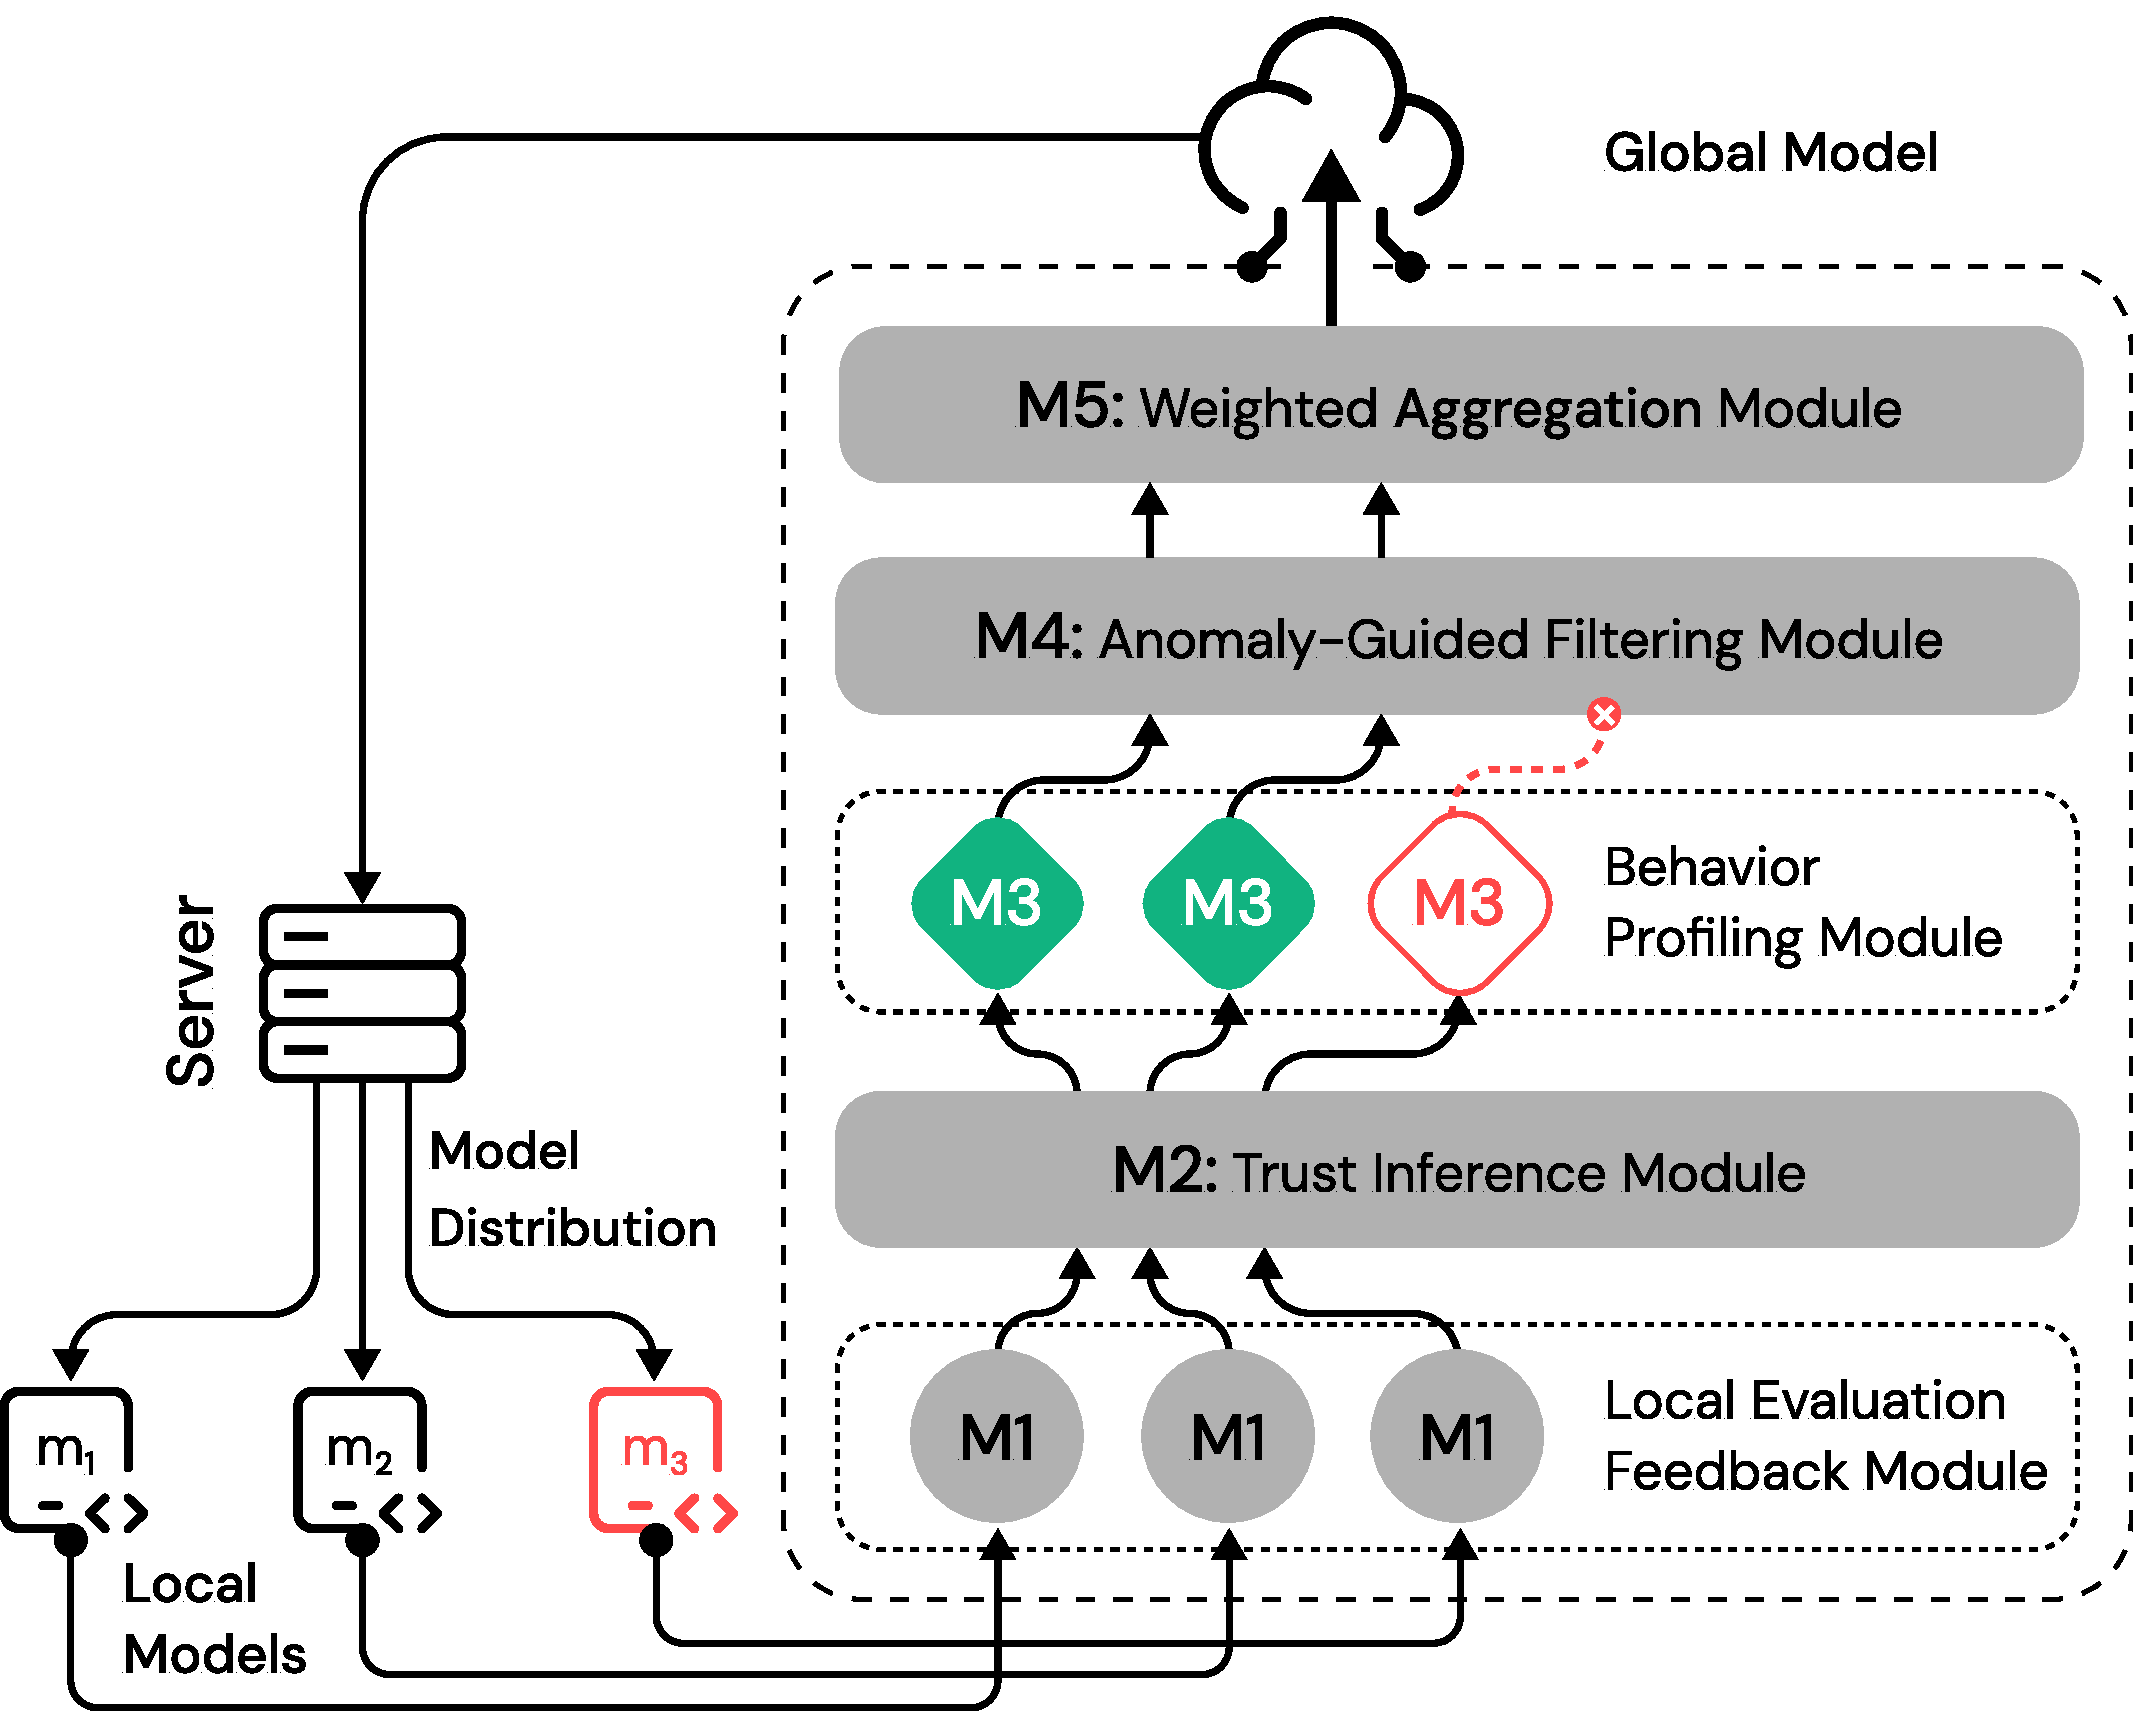
\includegraphics[height=0.75\columnwidth]{../fig/sys_arc.pdf}
  \caption{Workflow of the AntiFLipper Framework}
  \label{fig:sysArch}
\end{figure}
Each module operates within the standard FL loop, enhancing robustness against label-flipping attacks without altering the fundamental decentralized \textcolor{blue}{execution model}.

\subsection{M1: Local Evaluation Feedback Module}
At the beginning of each communication round, the server distributes the global model $M_i$ to all participating clients not in the malicious list $\beta$ (Algorithm~1, lines 2--3). 
In the reported full-evaluation runs, each client evaluates $M_i$ on its local training loader, computing a local accuracy score $acc_{ij}\in[0,1]$; no held-out local split is used, so evaluated samples can also be used for local training. Malicious clients use the same flipped labels for evaluation and training. \textcolor{blue}{Only this scalar is returned to the server; no raw data is transmitted.} Because $M_i$ primarily reflects honest labels, its accuracy on the systematically flipped labels provides the detection signal. Each client also trains a local model $m_{ij}$ and returns both $m_{ij}$ and $acc_{ij}$ to the server.

\subsection{M2: Trust Inference Module}
Upon receiving the results, the server computes the average accuracy across all non-malicious clients (i.e., excluding clients identified as malicious up to the current round) (Algorithm~\ref{alg:malfilter}, line~1). The trust score $\tau_j$, initialized uniformly as $1/N$ where $N$ is the total number of clients, is then updated for each client $j$ based on the squared deviation from the computed average:
$\tau_j \leftarrow \tau_j \pm \eta \cdot (acc_{avg} - acc_{ij})^2$.
Here, \texttt{sqDeviation()} $= (acc_{ij}-acc_{avg})^2$; \texttt{penalizeTrust()} $= \tau_j - \eta \cdot d$; and \texttt{rewardTrust()} $= \tau_j + \eta \cdot d$. The implementation clips negative trust to zero, assigns zero to already detected clients, and divides every remaining value by the sum over non-detected clients. It has no separate upper-clipping operation before normalization.
The sign is negative if $acc_{ij} < acc_{avg}$ (lines 4--5) and positive otherwise (lines 6--7). This quadratic penalty function penalizes deviations from the average more strongly than a linear scheme, addressing the issue where small but persistent differences could accumulate disproportionately over multiple rounds under a linear penalty formulation.


\IncMargin{1em}
\setlength{\textfloatsep}{0pt}
\begin{algorithm}[t]
  \caption{\texttt{AntiFLipper()}}\label{alg:antiflipper}
  \SetKwFunction{AntiFLipper}{AntiFLipper}
  \SetKwInOut{Input}{Input}
  \SetKwInOut{Output}{Output}
  \Indm 
    \Input{Number of clients $n$, client list $clients$, local datasets $data$, trust learning rate $\eta$, trust threshold $\tau_{\text{threshold}}$, flag threshold $cnt_{\text{max}}$}
    \Output{Global model $M_{i+1}$, malicious clients list $\beta$}
  \Indp
  \BlankLine

  $(M_0,\ \tau,\ cnt,\ \beta) \leftarrow \texttt{Initialize}()$\\

  \For{$i \leftarrow 1$ \KwTo $totalRounds$}{
        \texttt{DistributeModel}($M_{i}, clients,\ \beta$)\\
    \ForEach{$j \in clients$ \textbf{and} $j \notin \beta$}{
        $(m_{ij},\ acc_{ij}) \leftarrow \texttt{LocTrain}(M_i,\ j,\ data_{ij})$\\
    }
        $(\tau,\ cnt,\ \beta) \leftarrow \texttt{MalNodeFilter}(clients ,\ acc_{ij},\ \tau,\ cnt,\ \beta)$\\
    $M_{i+1} \leftarrow \texttt{GlobModelAgg}(m,\ \tau,\ clients,\ \beta)$\\
  }

  \Return{$M_{i+1},\ \beta$}
\end{algorithm}
\DecMargin{1em}

\subsection{M3: Behavior Profiling Module}
The server analyzes accuracy and trust scores over multiple rounds to build a behavior profile per client via the flag counter $cnt_j$ (Algorithm~2, lines 8--11), tracking how many rounds a client's trust has fallen below threshold. \textcolor{blue}{AntiFLipper makes no assumptions about data distribution or non-IID structure and uses relative performance deviations across clients for detection. It tolerates occasional accuracy drops from natural heterogeneity, penalizing only persistent anomalies, enabling robust detection without distribution-aware mechanisms.}

\textcolor{blue}{When malicious clients are few or their accuracy deviation is small, they may not be immediately flagged. This is a detection limitation even when their aggregate effect is modest, and motivates reporting identification metrics in future evaluations.}

\subsection{M4: Anomaly-Guided Filtering Module}
To avoid overreacting to a single accuracy drop, each client's flag counter $cnt_j$ tracks cumulative underperformance rounds and is not reset after a non-violating round. Beginning with the third communication round, a client whose trust is below the fixed implementation threshold $\tau_{\text{thresh}}=0.0005$ has its counter incremented (Algorithm~\ref{alg:malfilter}, lines 8--9). Once six violations have accumulated, the client is added to $\beta$ (lines 10--11), assigned zero trust, and omitted from aggregation in subsequent rounds. Trust values are normalized over the remaining clients (line 12). The fixed threshold is equivalent to $1/(20N)$ for the 100-client MNIST runs and $1/(100N)$ for the 20-client CIFAR-10 runs.

\IncMargin{1em}
\setlength{\textfloatsep}{0pt}
\begin{algorithm}[t]
  \caption{\texttt{MalNodeFilter()}}\label{alg:malfilter}
  \SetKwFunction{MalNodeFilter}{MalNodeFilter}
  \SetKwInOut{Input}{Input}
  \SetKwInOut{Output}{Output}
  \Indm 
    \Input{Clients $clients$, Accuracies $acc_{ij}$, Trust values $\tau$, Flags $cnt$, Malicious list $\beta$}
    \Output{Updated $\tau$, $cnt$, $\beta$}
  \Indp
  \BlankLine
  
  $acc_{avg} \leftarrow \texttt{getAvgAccuracy}(clients \setminus \beta)$\\
  
  \ForEach{$j \in clients$ \textbf{and} $j \notin \beta$}{
    
      $d \leftarrow \texttt{sqDeviation}(acc_{ij}, acc_{avg})$\\
      \If{$acc_{ij} < acc_{avg}$}{
        $\tau_j \leftarrow \texttt{penalizeTrust}(\tau_j, d, \eta)$\\
      }
      \Else{
        $\tau_j \leftarrow \texttt{rewardTrust}(\tau_j, d, \eta)$\\
      }

      \If{$\tau_j < \tau_{\text{thresh}}$}{
        $cnt_j \leftarrow cnt_j + 1$\\
        \If{$cnt_j \ge cnt_{\text{max}}$}{
          add $j$ to $\beta$\\
        }
      }
  }

  
      
    
  
  $\tau \leftarrow \texttt{normalizeTrust}(\tau, \beta)$\\

  \Return{$\tau$, $cnt$, $\beta$}
\end{algorithm}
\DecMargin{1em}
The overall malicious node filtering process is implemented in Algorithm 2, which is invoked from the main AntiFLipper algorithm (Algorithm 1, line 6) during each communication round, before global model aggregation.


 \subsection{M5: Weighted Aggregation Module}
After malicious clients have been filtered out, the remaining client models are aggregated using a weighted average (Algorithm 1, line 7). The weight assigned to each client's model is proportional to its normalized trust score. Formally, the aggregated model $M_{i+1}$ is computed as: \(
M_{i+1} = \sum_{j \in \text{Honest}} \frac{\tau_j}{W} \cdot m_{ij} \), where $W = \sum_{j \in \text{Honest}} \tau_j$. This gives higher-trust clients greater influence while suppressing clients that have been classified as malicious.

\section{Implementation and Evaluation}
\label{sec:implement&eval}

We developed AntiFLipper\footnote{The source code is available at: \url{https://github.com/abidh8820/AntiFlipper}} in Python and evaluated it under label-flipping attacks against established defenses, including FedAvg~\cite{fedavg-pmlr-v54-mcmahan17a}, Median, Trimmed Mean~\cite{yin2018byzantine}, FoolsGold~\cite{fung2020limitations}, Tolpegin~\cite{tolpegin2020data}, MKRUM~\cite{NIPS2017_f4b9ec30}, FLAME~\cite{nguyen2022flame}, and LFighter~\cite{jebreel2024lfighter}. Experiments were implemented in PyTorch on a 12th Gen Intel Core i9-12900K CPU, 128GB RAM, and NVIDIA RTX 3090 GPU running Ubuntu 22.04.4 LTS. We evaluated on two benchmark datasets: MNIST70K~\cite{MNIST-lecun1998gradient}, comprising 70,000 grayscale digit images (60K train, 10K test), and CIFAR-10~\cite{CIFAR-krizhevsky2009learning}, containing 60,000 color images across 10 classes (50K train, 10K test). MNIST uses a two-convolution/two-fully-connected-layer CNN with 21,840 trainable parameters, while the reported CIFAR-10 runs use ResNet18~\cite{resnet-he2016deep}.

Experiments were conducted under both IID and non-IID settings. For MNIST, we simulated 100 clients, all active every round, under an IID random-uniform split and, separately, under Dirichlet~\cite{ferguson1973bayesian} non-IID partitioning ($\alpha=1$), running for 200 communication rounds with 3 local epochs, batch size 64, and SGD (lr=0.01, momentum=0.9). For CIFAR-10, the saved configurations and logs use 20 clients, all active every round, in both IID and Dirichlet non-IID ($\alpha=1$) settings, trained over 100 rounds with 3 local epochs, batch size 32, and SGD (lr=0.01, momentum=0.9). All settings contain 40\% malicious clients and use a constant, full-label permutation: $0\leftrightarrow1$, $2\leftrightarrow3$, $4\leftrightarrow5$, $6\leftrightarrow7$, and $8\leftrightarrow9$. The mapping is fixed across malicious clients and rounds. The trust implementation uses $\eta=0.1$, $\tau_{\text{thresh}}=0.0005$, and $cnt_{\max}=6$ cumulative violations.

\begin{figure}[!h]
    \centering
    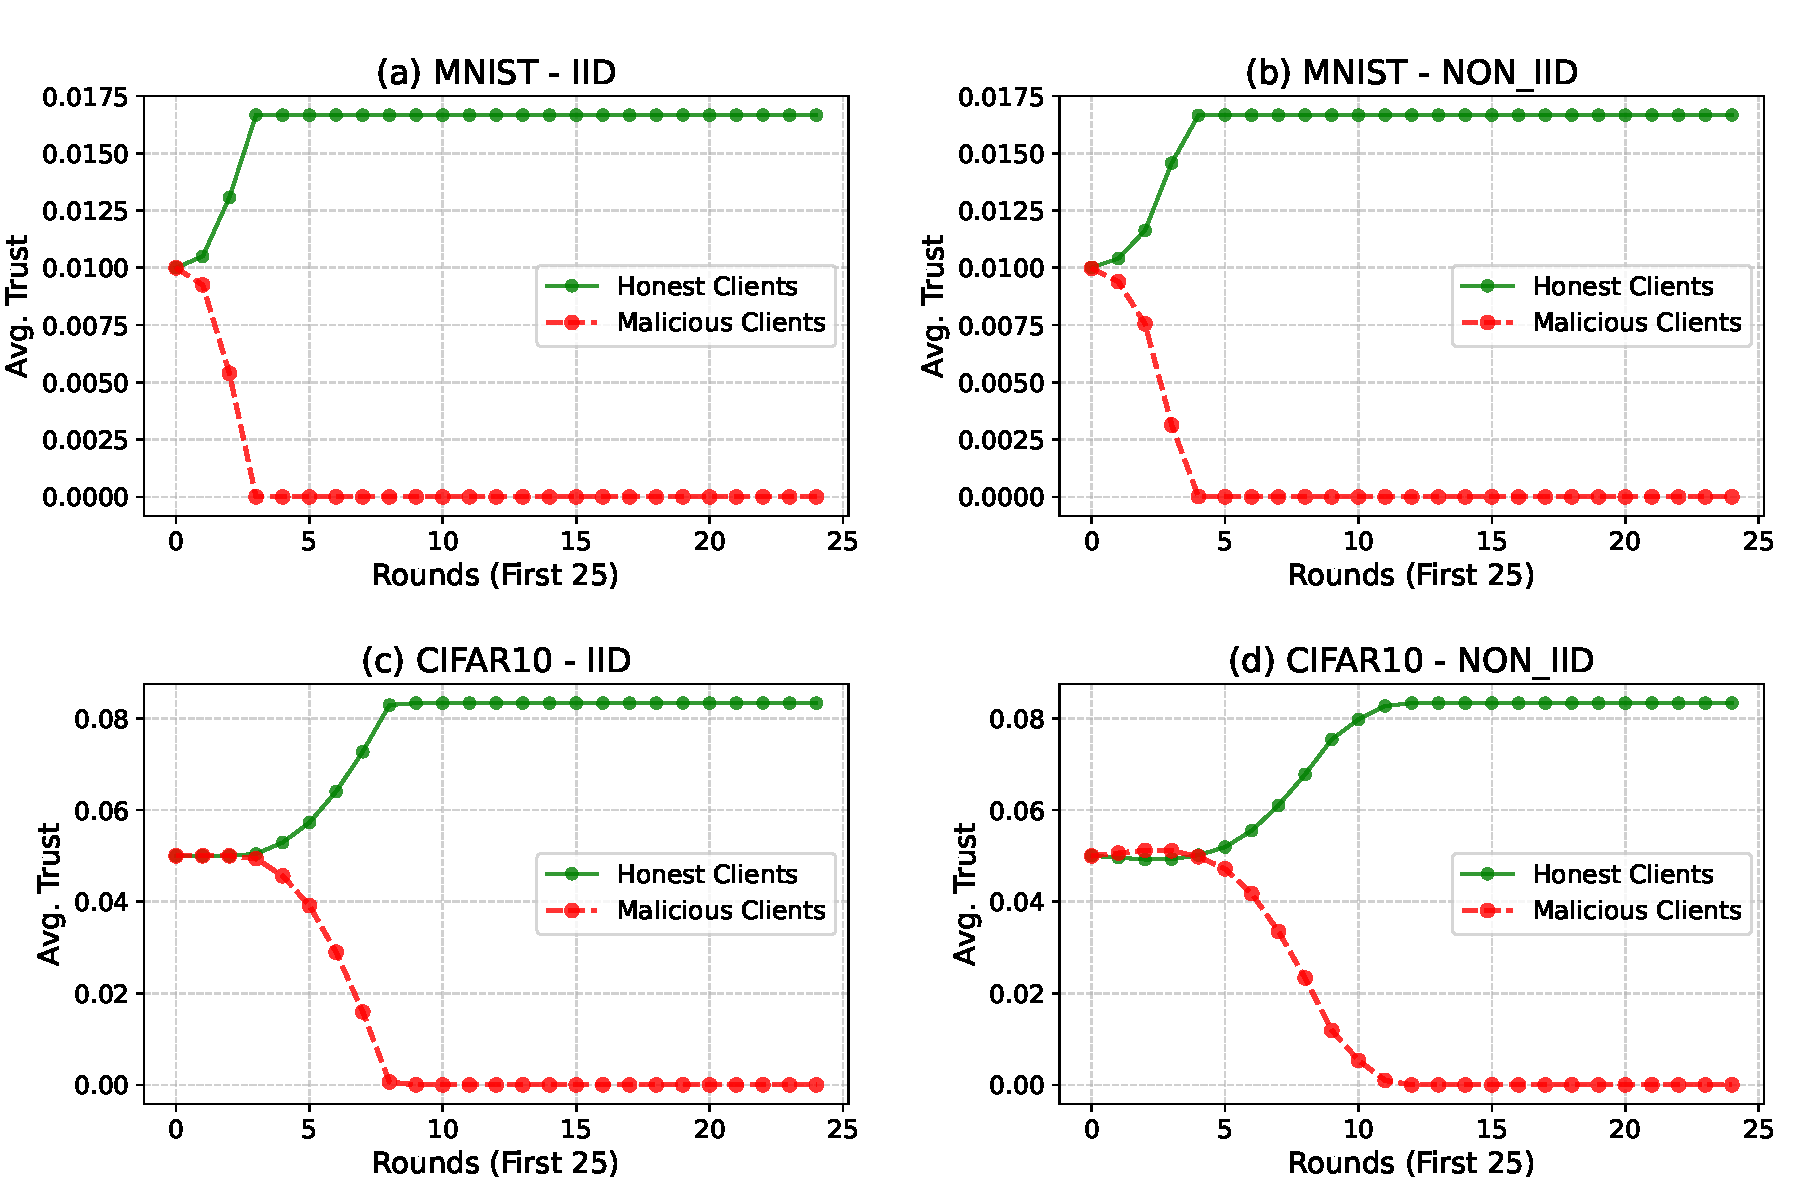
\includegraphics[width=1\linewidth]{../fig/antiflipper_combined_subplots_trust_updated.pdf}
    \caption{Average trust over clients in each detected-malicious or remaining-client group during the first 25 rounds.}
    \label{fig:Average Client Trust Over First 25 Rounds}
\end{figure}

\begin{table*}[tbh!] 
\centering 
\caption{\small Round-average results on MNIST and CIFAR-10 (IID and non-IID).} 
\renewcommand{\arraystretch}{1.2}
\scriptsize
\begin{tabular}{|c||p{3cm}||p{1.2cm}|p{1cm}|p{1cm}|p{1cm}|p{1cm}|p{1cm}|p{1cm}|p{1cm}|p{1.2cm}|} 
\hline
& \textbf{Methods} & \textbf{FoolsGold} & \textbf{FedAvg} & \textbf{Median} & \textbf{TMean} & \textbf{FLAME} & \textbf{MKRUM} & \textbf{LFighter} & \textbf{Tolpegin} & \shortstack{\textbf{Anti-}\\\textbf{FLipper}} \\
\cline{2-11} 
\hline\hline

\multirow{3}{*}{\rotatebox[origin=c]{90}{\shortstack{\textbf{MNIST} \\ \textbf{(IID)}}}} 
& \textbf{Global Accuracy (\%)}   & 0.36  & 51.85 & 96.10 & 96.18 & 97.44 & 97.45 & 97.45  & 97.45  & 97.06  \\ 
\cline{2-11}
& \textbf{Test Error}             & 17.60 & 0.86  & 0.18  & 0.18  & 0.09  & 0.09  & 0.09   & 0.09   & 0.10   \\ 
\cline{2-11}
& \textbf{Aggregation Time (ms)} & 9.36  & 4.61  & 12.03 & 12.86 & 45.61 & 15.55 & 119.65 & 160.94 & 3.01   \\ 
\hline\hline

\multirow{3}{*}{\rotatebox[origin=c]{90}{\shortstack{\textbf{MNIST} \\ \textbf{(NON-} \\ \textbf{IID)} }}} 
& \textbf{Global Accuracy (\%)}   & 3.58  & 53.99 & 95.67 & 95.61 & 97.03 & 96.74 & 96.76  & 96.80  & 96.77  \\ 
\cline{2-11}
& \textbf{Test Error}             & 6.72  & 0.76  & 0.22  & 0.23  & 0.11  & 0.12  & 0.13   & 0.13   & 0.11   \\ 
\cline{2-11}
& \textbf{Aggregation Time (ms)} & 8.65  & 4.44  & 13.09 & 11.73 & 45.66 & 13.70 & 119.37 & 168.88 & 2.96   \\ 
\hline\hline

\multirow{3}{*}{\rotatebox[origin=c]{90}{\shortstack{\textbf{CIFAR} \\ \textbf{(IID)}}}} 
& \textbf{Global Accuracy (\%)}   & 70.13 & 47.21 & 63.90 & 63.77 & 67.30 & 32.86 & 69.96  & 70.28  & 70.09  \\ 
\cline{2-11}
& \textbf{Test Error}             & 1.10  & 1.43  & 1.10  & 1.12  & 1.15  & 2.31  & 1.12   & 1.11   & 1.10   \\ 
\cline{2-11}
& \textbf{Aggregation Time (ms)} & 53.87 & 50.76 & 660.39 & 641.66 & 1489.91 & 686.93 & 468.02 & 354.96 & 48.01 \\ 
\hline\hline

\multirow{3}{*}{\rotatebox[origin=c]{90}{\shortstack{\textbf{CIFAR} \\ \textbf{(NON-} \\ \textbf{IID)} }}} 
& \textbf{Global Accuracy (\%)}   & 56.01 & 50.95 & 60.93 & 59.66 & 37.77 & 44.08 & 64.58  & 53.58  & 68.23  \\ 
\cline{2-11}
& \textbf{Test Error}             & 1.12  & 1.31  & 1.18  & 1.19  & 3.23  & 1.70  & 1.21   & 1.31   & 1.14   \\ 
\cline{2-11}
& \textbf{Aggregation Time (ms)} & 53.16 & 49.75 & 712.13 & 678.38 & 1334.06 & 727.38 & 449.12 & 339.47 & 48.43 \\ 
\hline\hline
\end{tabular} 
\label{table:result_table} 
\end{table*}

\subsection{Evaluation Metrics}
We evaluated using three metrics: global test accuracy, test error, and aggregation time. The first two are computed after every communication round on the standard centralized 10,000-example test set; Test Error is the arithmetic mean of per-batch cross-entropy loss. Each Table~\ref{table:result_table} entry is the arithmetic mean of the corresponding per-round sequence rather than the final or best round. Aggregation Time measures only the server-side aggregation code region.

\subsection{Malicious Node Detection}
AntiFLipper distinguishes malicious from honest clients using the global model's accuracy on local datasets. When a client flips labels, its local accuracy drops because the global model, trained primarily on honest labels, performs poorly on manipulated labels. The saved static-attack logs show exact recovery of the malicious set with no false positives: MNIST has 40 true positives, 0 false positives, and 0 false negatives (precision and recall 1.0), with all malicious clients detected by round 9 under IID and round 11 under non-IID. CIFAR-10 has 8 true positives, 0 false positives, and 0 false negatives, with all detected by round 15 under IID and round 18 under non-IID. Figure~\ref{fig:Average Client Trust Over First 25 Rounds} shows the corresponding group-average trust trajectories.

\subsection{Experimental Results}

On MNIST (Table~\ref{table:result_table}), AntiFLipper, LFighter, Tolpegin, MKRUM, FLAME, TMean, and Median all achieved high accuracy. FoolsGold collapsed in the non-IID setting (3.58\%), consistent with similarity-based defenses confusing heterogeneous honest updates. FedAvg amplified poisoned updates. AntiFLipper matched the evaluated robust defenses in accuracy while achieving the lowest measured aggregation time (3.01\,ms IID; 2.96\,ms non-IID), approximately 40 times faster than LFighter and 15 times faster than FLAME. \textcolor{blue}{The timer uses synchronized CUDA events around the aggregation branch and excludes local training, local evaluation, global testing, and data transfer; the table reports the mean over communication rounds. After detection, AntiFLipper aggregates updates from 60 rather than 100 clients on MNIST and 12 rather than 20 clients on CIFAR-10, whereas FedAvg retains every client. Consequently, AntiFLipper's slightly lower measured time than FedAvg reflects both its lightweight trust-weighted aggregation and the exclusion of detected clients.}

On CIFAR-10, results followed similar trends with generally lower accuracy. In IID, AntiFLipper (70.09\%) was close to LFighter, Tolpegin, and FoolsGold while recording the lowest aggregation time (48\,ms versus 1490\,ms for FLAME). In the tested non-IID configuration, AntiFLipper had the highest accuracy (68.23\%) among the evaluated methods and the lowest measured aggregation time. These results demonstrate the method on a more complex image dataset without a server-side reference dataset; both CIFAR-10 settings use the same 20-client, full-participation configuration.

We further tested AntiFLipper under two dynamic attack schedules: (1) attacks beginning after half of the total communication rounds and (2) poisoning once every 15 rounds. Table~\ref{table:dynamic_table} reports the resulting global test accuracies. Both schedules retained high MNIST accuracy and produced CIFAR-10 accuracies between 70.59\% and 72.66\%. %\textcolor{red}{[AUTHOR TO CONFIRM FROM LOGS: number of malicious clients detected, detection round, false positives, false negatives, and aggregation time for each dynamic scenario before claiming complete detection or unchanged efficiency.]}

\begin{table}[h]
\centering
\caption{Global test accuracies (\%) under dynamic attack scenarios}
\label{table:dynamic_table}
\begin{tabular}{|l||c|c|c|c|}
\hline
\textbf{Scenario} & \multicolumn{2}{c|}{\textbf{MNIST}} & \multicolumn{2}{c|}{\textbf{CIFAR-10}} \\
\cline{2-5}
 & \textbf{IID} & \textbf{Non-IID} & \textbf{IID} & \textbf{Non-IID} \\
\hline \hline
Scenario 1 & 96.93 & 97.03 & 72.66 & 70.62 \\ \hline
Scenario 2 & 96.68 & 96.82 & 72.59 & 70.59 \\
\hline
\end{tabular}
\end{table}

\begin{figure}[t]
    \centering
    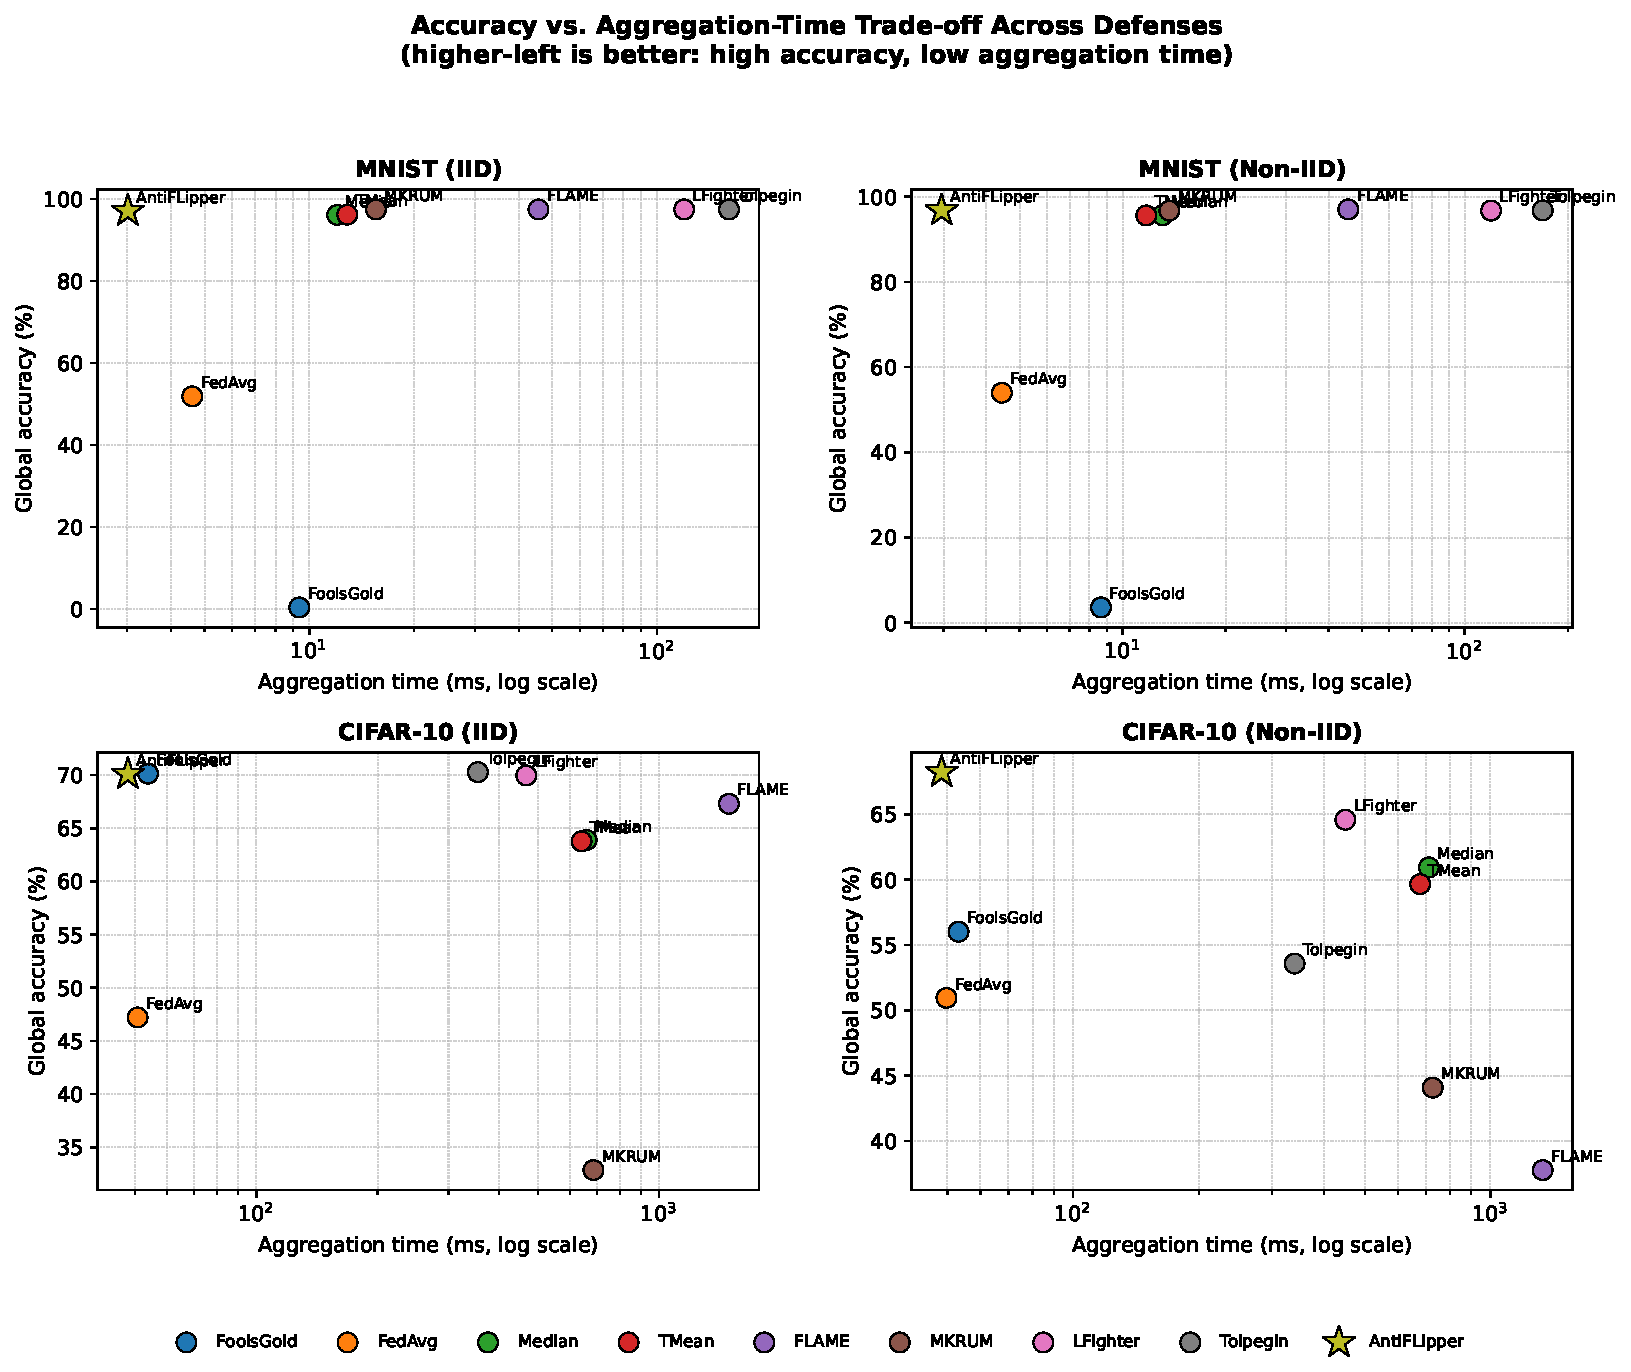
\includegraphics[width=1\linewidth]{accuracy_time_tradeoff.pdf}
    \caption{\textcolor{blue}{Accuracy vs.\ aggregation-time trade-off across all nine methods and four dataset/distribution settings (data as reported in Table~\ref{table:result_table}; note the log-scaled time axis). AntiFLipper (star) consistently occupies the upper-left region, matching the accuracy of the best-performing baselines while incurring the lowest aggregation time in every setting.}}
    \label{fig:tradeoff}
\end{figure}

\textcolor{blue}{Figure~\ref{fig:tradeoff} restates the results of Table~\ref{table:result_table} as an accuracy-versus-aggregation-time trade-off, which makes the practical value of AntiFLipper's design more directly visible than the raw table: across all four dataset/distribution settings, AntiFLipper sits in the upper-left region (high accuracy, low time), whereas the next most accurate defenses (LFighter, FLAME, Tolpegin) are shifted one to two orders of magnitude to the right on the log-scaled time axis.}

\noindent In summary, the reported runs show that AntiFLipper retains useful accuracy under the tested static and dynamic label-flipping conditions while keeping measured server-side aggregation time low.


\section{Security Analysis}
\label{sec:securityanalysis}

In this section, we formalize AntiFLipper’s trust-based defense against label-flipping attacks. Our approach quantifies deviations in local model accuracy to adjust client trust scores, enabling the system to progressively isolate and exclude malicious participants. This establishes AntiFLipper as an efficient and robust defense for secure federated learning in adversarial federated learning environments.

\subsection{Accuracy-Based Detection of Label Flipping Behavior} A key challenge in federated learning is mitigating label-flipping attacks, where malicious clients poison training by mislabeling data. AntiFLipper tackles this by exploiting the accuracy drop observed when the global model is trained on such poisoned data.

\textit{\textbf{Proposition 1 (detection signal under stated assumptions).} Suppose the global model \(M\) is dominated by honest updates and label flipping produces a persistent expected accuracy gap \(g_i=\mathbb{E}[\operatorname{acc}(M,d_H)]-\mathbb{E}[\operatorname{acc}(M,d_i')]>0\). Then the flipped client has a larger expected downward deviation from the population accuracy than a comparable honest client, providing a signal for AntiFLipper's trust update.} \\

\textit{\textbf{Justification:}} Let the expected accuracy on comparable honest clients be $a_H$ and on a flipped client be $a_M=a_H-g_i$. If a fraction $p$ of active clients is malicious and the server uses an unweighted mean accuracy, then $a_{avg}\approx(1-p)a_H+pa_M$. The expected downward deviations are $a_{avg}-a_M=(1-p)g_i$ for a malicious client and $a_{avg}-a_H=-pg_i$ for an honest client. AntiFLipper penalizes the former and rewards the latter before normalization. Repetition over rounds can therefore separate trust scores when $g_i$ remains positive and dominates sampling and non-IID variation. The proposition is conditional: neither higher cross-entropy loss nor label flipping alone guarantees lower 0--1 accuracy for every model and dataset. Severe heterogeneity, targeted partial flips, or a sufficiently corrupted global model can violate the assumed gap, as discussed below.

\subsection{Trust Score Convergence for Malicious Exclusion}
\textit{\textbf{Proposition 2 (finite filtering under persistent low trust).} If a client's normalized trust satisfies \(\tau_i\leq\tau_{\text{thresh}}\) in at least $cnt_{\max}$ counted rounds, Algorithm~\ref{alg:malfilter} adds it to $\beta$ no later than the $cnt_{\max}$-th such round.} \\

\textit{\textbf{Proof:}} The counter is initialized at zero and increases by one whenever the threshold condition holds. Algorithm~\ref{alg:malfilter} adds the client to $\beta$ when $cnt_i\geq cnt_{\max}$; hence the claim follows directly. This proposition establishes termination of the filtering rule under persistent low trust, not that every filtered client is malicious or that every malicious client will cross the threshold. Those identification properties depend on Proposition~1's accuracy-gap assumption and on the choices of $\eta$, $k$, and $cnt_{\max}$.

\subsection{Dependence on the Malicious Client Ratio}
\label{sec:ratioanalysis}
\textcolor{blue}{Proposition~1 rests on the assumption that $M$ is aggregated predominantly from honest updates, so that its decision boundaries reflect the honest label distribution rather than the flipped one. Let $p \in [0,1]$ denote the fraction of participating clients that are malicious in a given round, and let $\text{acc}_H$ and $\text{acc}_{M'}$ denote the global model's expected accuracy on honest and flipped data, respectively, before any exclusion. Approximating the unweighted mean across clients gives $\text{acc}_{avg} \approx (1-p)\cdot \text{acc}_H + p \cdot \text{acc}_{M'}$, so the detectable gap for a malicious client shrinks as
\[
\text{acc}_{avg} - \text{acc}_{M'} \;\approx\; (1-p)\,(\text{acc}_H - \text{acc}_{M'}),
\]
which is monotonically decreasing in $p$ for a fixed positive $\text{acc}_H-\text{acc}_{M'}$ and vanishes as $p \to 1$. As the malicious fraction grows, $M$ may also become increasingly shaped by poisoned updates, further reducing the underlying accuracy gap. Our experiments evaluate a 40\% malicious ratio, which lies within Multi-Krum's admissible regime for the tested client counts~\cite{NIPS2017_f4b9ec30}.}

\subsection{Robustness to Non-IID Skew and Adaptive Adversaries}
\textcolor{blue}{The flag-counter mechanism (M4) safeguards against penalizing honest clients whose accuracy is transiently low due to non-IID skew: a low-trust round increments $cnt_j$, while exclusion requires $cnt_{\max}$ cumulative violations. A persistently skewed honest client could still be misclassified if its trust remains below $\tau_{\text{thresh}}$ long enough; the evaluated non-IID setting uses Dirichlet $\alpha=1$.}

\subsection{Privacy Considerations of Accuracy Reporting}
\textcolor{blue}{While AntiFLipper avoids transmitting raw data or gradients, the scalar $acc_{ij}$ is not information-free: repeated accuracy reports across rounds implicitly reveal how well the evolving global model fits a client's local distribution, which could in principle support membership-inference-style reasoning about a client's data composition, particularly for clients with small or highly unique local datasets. This risk is qualitatively smaller than gradient- or update-based leakage (the object exploited by classical FL membership-inference attacks), since a single scalar carries far less information than a full model update, but it is not zero. A standard mitigation would be to inject calibrated noise into $acc_{ij}$ before transmission, e.g., via a Laplace or Gaussian mechanism sized to a target $(\epsilon,\delta)$-differential-privacy budget, analogous to the noise-addition step used by FLAME~\cite{nguyen2022flame} for its clustering inputs. Because the trust update (Section~\ref{sec:methodology}, M2) already operates on a \emph{squared deviation} from a population average rather than the raw value, we expect it to be reasonably tolerant of small additive noise, but quantifying the resulting privacy-utility trade-off (i.e., how much noise the detector can absorb before its recall degrades) requires a dedicated empirical study that we leave to future work rather than claim here.}

\subsection{Convergence Under Progressive Client Exclusion}
\textcolor{blue}{Progressive exclusion and trust reweighting prevent a direct claim that AntiFLipper inherits a standard FedAvg convergence theorem. M5 is a convex combination of surviving client models, but the client set and weights are history-dependent; false-positive exclusions can also change the optimized population objective and increase bias. Existing FedAvg analyses under bounded heterogeneity~\cite{li2020convergence} describe the fixed-objective baseline but do not directly prove convergence of this filtering process. The stable accuracy trajectories summarized in Tables~\ref{table:result_table} and~\ref{table:dynamic_table} provide empirical evidence for the tested settings only. A formal analysis would need assumptions bounding honest-client false exclusions, weight variation, and gradient dissimilarity over the surviving set.}


\section{Computational and Communication Overhead of AntiFLipper}
\label{sec:overhead}

To quantify the computational overhead introduced by local evaluation in {AntiFLipper}, we consider a neural network model $f(x; w)$ with $W$ parameters, trained on each client $k$ with dataset $D_k$ of $n_k$ samples. Clients perform $E$ local SGD epochs (batch size $B$), where the per-sample forward and backward pass costs are $C_f$ and $C_b \approx 2C_f$, respectively. Thus, the training cost per client per round is $C_{\text{train}} \approx 3E \cdot n_k \cdot C_f$.

Local evaluation on a fraction $\gamma$ of the data adds $C_{\text{eval}} = \gamma \cdot n_k \cdot C_f$, leading to a total cost of $C_{\text{total}} = n_k \cdot (3E + \gamma) \cdot C_f$, and relative overhead $\frac{\gamma}{3E}$. In our experiments with $E = 3$, full evaluation ($\gamma = 1$) yields a worst-case overhead of ~11.1\%. The global accuracies reported in Table~\ref{table:result_table} correspond to this full local data evaluation setting.

To reduce cost, we also evaluated the global model on only 10\% of each client's local data ($\gamma = 0.1$), giving an analytical evaluation overhead of approximately 1.1\% relative to three local training epochs. The resulting global accuracies were $97.11\%$ (MNIST IID), $96.79\%$ (MNIST non-IID), $74.81\%$ (CIFAR-10 IID), and $68.18\%$ (CIFAR-10 non-IID), demonstrating that reduced local evaluation can preserve competitive global accuracy while lowering client-side evaluation cost.

\textcolor{blue}{AntiFLipper avoids server-side inspection of updates, eliminating the main overhead in competing methods. Instead of FLAME-style aggregation, it shifts evaluation to clients in parallel, keeping aggregation lightweight and scalable. The parameter $\gamma$ provides a flexible trade-off between efficiency and detection sensitivity.}

\subsection{Communication Overhead}
\textcolor{blue}{Beyond computation, we analyze communication cost. In each round, every participating client downloads the global model ($W$ parameters) and uploads its locally trained model update (also $W$ parameters), as in vanilla FedAvg~\cite{fedavg-pmlr-v54-mcmahan17a}; AntiFLipper adds the scalar $acc_{ij}$, represented here as one 32-bit float (4 bytes), to the upload. With 32-bit model parameters, this is a fractional overhead of $1/W$ relative to the upload payload, or approximately $1/(2W)$ relative to the combined model download and update upload, ignoring protocol metadata. For the 21,840-parameter MNIST CNN, the added fractions are approximately $0.00458\%$ of the upload and $0.00229\%$ of combined download and upload. Cryptographic defenses such as Shen et al.~\cite{shen2024lfrppfl} incur encryption-related computation and representation overhead, while server-reference-based methods such as FLTrust~\cite{cao2020fltrust} and HSCS~\cite{li2023hscs} require a clean server dataset. FLAME~\cite{nguyen2022flame} and other clustering-based defenses need not add client payload, but incur server-side processing over the received updates.}


\section{Limitations and Threats to Validity}
\label{sec:limitations}
\textcolor{blue}{AntiFLipper is evaluated as a computationally efficient client-side detection mechanism for label-flipping attacks. The following points define the scope within which the reported results should be interpreted:}

\begin{itemize}
    \item \textcolor{blue}{\textbf{Evaluation setting.} The experiments cover MNIST and CIFAR-10 with CNN and ResNet18 models, a 40\% malicious-client ratio, and Dirichlet $\alpha=1$ for non-IID data. The reported conclusions apply to these settings.}
    \item \textcolor{blue}{\textbf{Threat model.} The defense targets label manipulation under a trusted accuracy-reporting mechanism. Attackers that can falsify reports, arbitrarily modify model updates, or compromise the evaluation module fall outside this threat model.}
    \item \textcolor{blue}{\textbf{Deployment setting.} Experiments use synchronous participation and workstation-class hardware. The analytical overhead results motivate edge deployment, while actual latency depends on the target device and communication environment.}
\end{itemize}

\textcolor{blue}{These boundaries separate the claims supported by the present experiments from broader Byzantine, adaptive, and deployment-level settings.}

\section{Conclusion}
\label{sec:conclusion}

In this paper, we introduced AntiFLipper, a lightweight mechanism for detecting and mitigating label-flipping attacks in federated learning. Across the evaluated IID and non-IID settings on MNIST and CIFAR-10, AntiFLipper matched or exceeded the accuracy of the tested defenses while requiring substantially less measured server-side aggregation time than the more computationally intensive baselines. Its additional communication consists of one accuracy scalar per participating client. These results establish a promising security--efficiency trade-off under the stated label-flipping threat model and motivate evaluation across additional attack, data, and deployment settings.


\bibliographystyle{IEEEtran}
\bibliography{IEEEabrv,bibliography_updated}
\end{document}
